\section{Preparing trial balances}
\label{sec:trial}

\begin{definition}
    {Trial balance}
    An accounting report showing the closing balances of all general ledger accounts.

    Their purpose is to ensure that the \underline{debits and credits are equal} - to check for errors and help prepare financial statements.
\end{definition}

\small
\begin{tcolorbox}[colframe=black,colback=white,title=Example Trial Balance]
    \begin{center}
        \textbf{XYZ Corporation}\\
        \textbf{Trial Balance}\\
        For the period ended December 31, 2025\\
        (In millions of dollars)
    \end{center}
    \begin{tabular}{lrr}
        \textbf{Account} & \textbf{Debit} & \textbf{Credit} \\
        \hline
        Cash             & \$1,000        &                 \\
        Common Stock     &                & \$1,000         \\
        \hline
        \textbf{Total}   & \$2,000        & \$2,000         \\
    \end{tabular}
\end{tcolorbox}
\normalsize

\subsection{Posting adjusting entries}
\label{subsec:post_adjust}

\begin{theorem}
    {Adjusting our Trial Balance}
    In the account cycle, after preparing an unadjusted trial balance, we make adjustments to respect the \hyperref[thm:accrual_basis]{Accrual Basis of Accounting} for different types of expense and revenues.

    This adjustment is necessary when the two sides of a transaction (remember \hyperref[thm:debit_credit]{double-sided nature}) happens in a \underline{different accounting period}. (So no adjustments necessary if same period)
\end{theorem}

\begin{theorem}
    {A typical transaction}
    In a transaction there are two parties: a buyer and a seller.

    Seller $\xrightleftharpoons[\text{cash}]{\text{services}}$ Buyer

    In the case of the \textbf{buyer}, the transaction will always be an \textbf{expense}.

    In the case of the \textbf{seller}, the transaction will always be \textbf{revenue}.
\end{theorem}

\begin{definition}
    {Categorizing E\&R as prepayments / accruals}
    We need to categorize E\&R as either \textbf{Prepayments} or \textbf{Accruals} before making an adjusting entry as part of the analysis.
    \begin{itemize}
        \item \textbf{Prepayments}: services paid for before received (by buyer), also called \textbf{Deferrals}
        \item \textbf{Accrued}: services received before paid for (by buyer)
    \end{itemize}

\end{definition}

Hence, there will be \textit{4 titles} for the adjusting entries as follows, along with examples:
\begin{itemize}
    \item \textbf{Deferred Expense} (A, Dr)\\
          \textit{Example}: As a buyer, you drive a car. Your car warranty is for a year, but you pay for it the year prior. The service (car warranty) is paid for before received, hence, this is a prepaid expense.

          \vspace{1em}
    \item \textbf{Deferred Revenue} (L, Cr)\\
          \textit{Example}: As a seller, you sell car warranty. The service (car warranty) is paid for by the customer before it becomes active in the next year, hence, this is a deferred (prepaid) revenue.

          \vspace{1em}
    \item \textbf{Accrued Expense} (L, Cr)\\
          \textit{Example}: As a buyer, you consume water. Water bills are paid every 3 months, but you use water every month and your accounting period is a month. The service (water) is received before paying for by the customer, hence, this is an accrued expense.

          \vspace{1em}
    \item \textbf{Accrued Revenue} (A, Dr)\\
          \textit{Example}: As a seller, you provide water. The service (water) is provided before paying for by the customer, hence, this is an accrued revenue.

          \vspace{1em}
\end{itemize}

\begin{theorem}
    {What the adjusting entry does}
    As we recorded our transaction on the cash basis initially, it \textbf{overstates} the corresponding E/R. The purpose of the adjusting entry is to \textbf{correct this overstatement} by converting the transaction to either \textbf{A/L}. This conversion moves the transaction to the \hyperref[def:temp_perm]{\textbf{permanent accounts}}, which carries forward to the next period for adjustment again.

    To determine if the overstated transaction is A/L:
    \begin{itemize}
        \item \textbf{Asset (Dr)}: Future economic benefit
        \item \textbf{Liability (Cr)}: Future economic sacrifice
    \end{itemize}
    \label{thm:adjusting_entry}
\end{theorem}

\begin{theorem}
    {Releasing prepayments and accruals}
    As we record by the accrual basis, when we consume the / a part of the service, or the payment is made, we need to record the transaction accordingly. If only a part of the service is consumed, \underline{calculate the consumed amount by time period}.

    This moves the transaction back to the \hyperref[def:temp_perm]{\textbf{temporary accounts}}.
\end{theorem}
\label{thm:release}

\begin{knBox}
    {Summary}
    \begin{center}
        \begin{tabular}{c|c|c|c}
            Dr & Cr & Cr & Dr \\
            \hline
            DE & DR & AE & AR \\
        \end{tabular}

        \begin{tikzpicture}[overlay, remember picture]
            % Draw the line
            \draw[thick] (-1.5,0) -- (-1.5,-0.25) -- (0.5,-0.25) -- (0.5,0);
            % Add the label
            \node at (-0.5, -0.5) {Buyer};
            % Draw the line
            \draw[thick] (0.6,-0.25) -- (0.6,-0.5) -- (1.5,-0.5) -- (1.5,-0.25);
            % Add the label
            \node at (1, -1) {Received before paid for};
        \end{tikzpicture}

        \vspace{3em}
    \end{center}
\end{knBox}

\small
\begin{tcolorbox}[colframe=black,colback=white,title=Example Adjusting Entry (Prepaid Expense)]
    We make the following adjusting entry for car warranty (example above) that we paid for in the month prior.

    \vspace{1em}
    \begin{tabular}{llll}
        \textbf{Date} & \textbf{Account}      & \textbf{Dr} & \textbf{Cr} \\
        \hline
                      & \textit{in thousands} &             &             \\
        Dec 31, 2023  & Prepaid expense       & \$12        &             \\
                      & \quad Cash            &             & \$12        \\
    \end{tabular}
    \vspace{1em}

    Then each month, we will make the following adjusting entry to recognize the usage of the prepaid expense and release it gradually.

    \vspace{1em}
    \begin{tabular}{llll}
        \textbf{Date} & \textbf{Account}      & \textbf{Dr} & \textbf{Cr} \\
        \hline
                      & \textit{in thousands} &             &             \\
        XXX 31, 2024  & Utility expense       & \$1         &             \\
                      & \quad Prepaid expense &             & \$1         \\
    \end{tabular}
    \vspace{1em}
\end{tcolorbox}

\begin{tcolorbox}[colframe=black,colback=white,title=Example Adjusting Entry (Accrued Expense)]
    We make the following adjusting entry for water bills (example above) in the first and second month. By the history average, we assume each month costs around \$1000.

    Remember that \textit{accrued expense} is a \textbf{liability}, as it would be a future economic sacrifice.

    \vspace{1em}

    \begin{tabular}{llll}
        \textbf{Date} & \textbf{Account}                                   & \textbf{Dr} & \textbf{Cr} \\
        \hline
                      & \textit{in thousands}                              &             &             \\
        Jan 31, 2023  & Utility expense                                    & \$1         &             \\
                      & \quad Accrued expense                              &             & \$1         \\
                      & \multicolumn{3}{l}{\textit{(Water bills accrued)}}                             \\
        Feb 28, 2023  & Utility expense                                    & \$1         &             \\
                      & \quad Accrued expense                              &             & \$1         \\
                      & \multicolumn{3}{l}{\textit{(Water bills accrued)}}                             \\
    \end{tabular}
    \vspace{1em}

    We get the receipt for the water bills in the end of the third month. It was \$4. We record the utility expense and cash usage accordingly, then \hyperref[thm:release]{release} the accrued expense.

    \vspace{1em}
    \begin{tabular}{llll}
        \textbf{Date} & \textbf{Account}                                       & \textbf{Dr} & \textbf{Cr} \\
        \hline
                      & \textit{in thousands}                                  &             &             \\
        Mar 31, 2023  & Utility expense                                        & \$4         &             \\
                      & \quad Cash                                             &             & \$4         \\
                      & \multicolumn{3}{l}{\textit{(Water bills payment)}}                                 \\
        Mar 31, 2023  & Accrued expense                                        & \$2         &             \\
                      & \quad Utility expense                                  &             & \$2         \\
                      & \multicolumn{3}{l}{\textit{(Release accrued expense)}}                             \\
    \end{tabular}
\end{tcolorbox}
\normalsize

\subsection{Depreciation}
\label{subsec:depreciation}

\subsubsection{Recording as adjusting entry}

\begin{definition}
    {Depreciation}
    The process of reducing the book value of a tangible fixed asset over time.
\end{definition}

\begin{knBox}
    {Recording depreciation expense}
    \vspace{1em}
    \begin{tabular}{llll}
        \textbf{Date} & \textbf{Account}               & \textbf{Dr} & \textbf{Cr} \\
        \hline
        Dec 31, 2023  & Depreciation expense           & \$12        &             \\
                      & \quad Accumulated depreciation &             & \$12        \\
    \end{tabular}

    \vspace{1em}

    Accumulated depreciation is a \hyperref[def:contra]{\textbf{contra asset}}, as it has a normal balance opposite to the asset. We record it like the following in the balance sheet:

    \vspace{1em}

    \begin{tabular}{lr}
        \textbf{Assets}                &                                       \\
        \hline
        Equipment                      & \$100                                 \\
        \quad Accumulated depreciation & (12)                                  \\
        \hline
        \textbf{Total}                 & \$88 $\leftarrow$ \textbf{Book value} \\
    \end{tabular}

    Depreciation expense is an \textbf{operating expense}, as the depreciation occurs in the course of the business operations.
\end{knBox}

\begin{knBox}
    {Depreciation expense}
    The expense that is recorded \textbf{each period} over the useful life of the asset.
\end{knBox}

\subsubsection{Calculating depreciation expense}

Before calculation, you need to identify \textit{some} of the following quantities:
\begin{itemize}
    \item \textbf{(C) Cost}: The initial cost of the asset.
    \item \textbf{(RV) Residual value}: The estimated value of the asset at the end of its useful life.
    \item \textbf{(UL) Useful life}: The estimated number of years the asset will be used.
    \item \textbf{(P$_T$) Total production}: The total number of units the asset will produce over its useful life.
    \item \textbf{(P$_A$) Annual production}: The number of units the asset will produce in a year.
    \item \textbf{(AD) Accumulated depreciation}: The total depreciation expense recorded for the asset up to the current period.
\end{itemize}

\begin{theorem}
    {Depreciation estimation methods}
    \begin{tabular}{|p{0.2\textwidth}|p{0.3\textwidth}|p{0.3\textwidth}|}
        \hline
        \textit{Method}          & \textit{Formula}                            & \textit{Per period}                        \\
        \hline
        Straight-line            & \[\frac{C - RV}{UL}\]                       & Constant amount each period.               \\
        \hline
        Units-of-production      & \[(C - RV)\times\frac{P_A}{P_T}\]           & Based on production level.                 \\
        \hline
        Double-declining balance & \[2 \times \text{Straight line} \times AD\] & Double the straight-line rate each period. \\
        \hline
    \end{tabular}
\end{theorem}

Related: \hyperref[subsec:asset_disposal]{Asset disposal}

\subsection{Amortization}

\begin{definition}
    {Definite and indefinite life of intangible assets}
    When an intangible asset is aquired, managers will decide if they have a \textbf{definite} or \textbf{indefinite} life.
    \begin{itemize}
        \item \textbf{Definite life}: Cost is amortized over it's useful life across account periods.
        \item \textbf{Indefinite life}: Cost is not amortized, but tested for impairment annually.
    \end{itemize}
\end{definition}

\begin{knBox}
    {Amortization expense}
    The value is usually calculated by the \textbf{straight-line method}, similar to depreciation but without $RV$:
    \[\text{Amortization expense} = \frac{\text{C}}{\text{UL}}\]
\end{knBox}

\begin{knBox}
    {Impairment and impairment loss}
    Impairment is the reduction of an asset's value.
    \[\text{Impairment loss} = \text{Carrying value} - \text{Fair value}\]
\end{knBox}


\subsection{Sales revenue \& Bad debt expenses}

\subsubsection{Net sales revenue}

When considering the net sales revenue, we need to recognize some of the following deductions. They are not expenses, but a \hyperref[def:contra]{\textbf{contra revenue}} of \textbf{credit sales revenue}.

The following are three common contra accounts of sales revenue. When they occur, we \textbf{debit} the contra revenue account and \textbf{credit} sales revenue.

\begin{theorem}
    {Credit card discount}
    When paying with a credit card, the merchant will be charged a fee by the credit card company. This fee is typically a percentage of the transaction amount.
\end{theorem}

\begin{theorem}
    {Sales discounts}
    Discounts given to customers for early payment, called a \textbf{early repayment incentive}. For the following terms:
    \[2/10, n/30 \implies \text{2\% discount if paid within 10 days, otherwise net due in 30 days}\]
\end{theorem}

\begin{theorem}
    {Sales returns and allowances}
    Discounts given to customers for price discounts, or the total sales price of the returned goods.
\end{theorem}

\begin{knBox}
    {Presenting in income statement}
    We simply present as a \hyperref[def:contra]{\textbf{contra revenue}} of \textbf{sales revenue}.

    \begin{tabular}{lccc}
        \textbf{Sales revenue}             & \$1000           \\
        \quad Sales returns and allowances & (100)            \\
        \quad Sales discounts              & (50)             \\
        \quad Credit card discount         & \underline{(20)} \\
        \textbf{Net sales revenue}         & \$830            \\
    \end{tabular}
\end{knBox}

\subsubsection{Bad debts}

To keep track of each customer's account receivables, we usually assign an individual account for each customer (a \textbf{subsidiary account}).

\textbf{Bad debts} result from credit customers who will not pay the amount they owe (accounts receivable), regardless of collection efforts. For example, a customer who is bankrupt.

\begin{definition}
    {Account: Bad debt expense}
    An expense account for the amount of money that is not likely to be paid. There are two methods to do so:
\end{definition}


\subsubsection{Accounting bad debt expenses}

\begin{definition}
    {Account: Allowance for doubtful accounts}
    An \hyperref[def:contra]{\textbf{contra account}} for the \textbf{accounts receivable} to estimate the amount of money that will not be paid.
\end{definition}

\begin{theorem}
    {Credit sales}
    Credit sales are \textit{sales revenue} that \textbf{debit accounts receivable} (credit sales is not an account).
\end{theorem}

\begin{knBox}
    {Write-offs \& estimating bad debt expense}
    We record an \hyperref[thm:bad_debt_est]{\textbf{estimated}} bad debt expense at the end of the period of the credit sales as an adjusting entry.

    \vspace{0.3em}

    During the next period, we \textbf{write-off} the bad debt expense of the previous period, when we have \textbf{confirmed} that the customer will not pay, by deducting from \textbf{accounts receivable} to \textbf{allowance for doubtful accounts}.

    \vspace{0.3em}

    \textit{A write-off has no effects on the \textbf{net income}, as it is already recorded as an expense in the previous period.}

    \begin{itemize}
        \item End of period of sales: Allowance (\textbf{Cr}) $\rightarrow$ Bad debt expense (\textbf{Dr})
        \item Next period write-offs (confirmed bad debts): Accounts receivable (\textbf{Cr}) $\rightarrow$ Allowance (\textbf{Dr})
    \end{itemize}

\end{knBox}

\begin{knBox}
    {Recoveries}
    When a customer who has a bad debt previously pays, we simply revert the write-off entry:

    \vspace{1em}

    \begin{tabular}{llll}
        \textbf{Date} & \textbf{Account}                      & \textbf{Dr} & \textbf{Cr} \\
        \hline
        Dec 31, 2023  & Cash                                  & \$12        &             \\
                      & \quad Allowance for doubtful accounts &             & \$12        \\
    \end{tabular}
\end{knBox}

There are two methods to estimate the bad debt expense:
\begin{itemize}
    \item \textbf{Percentage of sales}
    \item \textbf{Aging method}
\end{itemize}
\label{thm:bad_debt_est}

\begin{theorem}
    {Estimate bad debt by Percentage of sales}
    Bad debt expense adjustment = \textbf{Credit} sales revenue (minus returns and allowances) $\times$ \textit{Historial} loss rate
\end{theorem}

\begin{theorem}
    {Estimate bad debt by Aging method}
    We estimate the \textbf{ending balance} of the allowance by the age of receivables, and calculate the adjustment by finding the \textbf{difference} between the allowance's \textbf{current balance} (beg. bal. of allowance - write-offs) and the ending balance.

    \begin{tabular}{lccc}
        \textbf{Age of receivable}                   & \textbf{Amount} & \textbf{Estimated loss rate} & \textbf{Estimated loss} \\
        \hline
        0-30 days                                    & \$1000          & 1\%                          & \$10                    \\
        31-60 days                                   & \$2000          & 2\%                          & \$40                    \\
        61-90 days                                   & \$1500          & 3\%                          & \underline{\$45}        \\
        \textbf{Estimated ending bal. of allowances} &                 &                              & \$95                    \\
        Balance of allowance                         &                 &                              & (\$5)                   \\
        \textbf{Bad debt expense adjustment}         &                 &                              & \$90                    \\
    \end{tabular}
\end{theorem}

\begin{knBox}
    {Presenting in income statement}
    We present the allowance of doubtful accounts as a \hyperref[def:contra]{\textbf{contra asset}} of \textbf{accounts receivable}.

    \begin{tabular}{lccc}
        \textbf{Accounts receivable}          & \$1000 \\
        \quad Allowance for doubtful accounts & (10)   \\
        \textbf{Net realizable value}         & \$990  \\
    \end{tabular}
\end{knBox}

